\documentclass{beamer}

\usepackage{xcolor}
\usepackage{graphicx}
\usepackage{tcolorbox}
\usepackage{listings}
\usepackage{booktabs}
\usepackage{array}
\usepackage{tabularx}

\usetheme{metropolis}

\begin{document}
\newcommand{\tabitem}{~~\llap{\textbullet}~~}

\lstset{
    basicstyle=\scriptsize\ttfamily,
    tabsize=4, % tab space width
    showstringspaces=false, % don't mark spaces in strings
    commentstyle=\color{grey}, % comment color
    keywordstyle=\color{blue}, % keyword color
    stringstyle=\color{purple} % string color
}

\title{Introduction to Programming}
\subtitle{Pointers and the STL Library}

\maketitle

\section{Memory, Pointers \& Reference}

\begin{frame}
    \frametitle{What is Memory?}

    \begin{itemize}
        \item Memory $\neq$ Storage
        \item Evolution in perspective:
            \begin{itemize}
                \item[--] Were data is stored.
                \item[--]<2-> A physical component that allows us to store data.
                \item[--]<3-> Is an abstraction that allows us to manage the physical components in a way we can understand.
            \end{itemize}
        \item How we think of memory \textbf{drastically} affects how we approach it.
    \end{itemize}

\end{frame}

\begin{frame}
    \frametitle{Accessing Memory}

    \setlength{\tabcolsep}{8pt}
    \begin{tabular}{ m{0.7\linewidth} m{0.2\linewidth} }
        \setlength{\tabcolsep}{0pt}
        \begin{tabular}{p{5mm} p{0.9\linewidth}}
            \tabitem & The smallest unit of memory we can access is called a \textit{byte}.\\
            \tabitem & Memory can be seen as a \textbf{HUGE} array of bytes, each with an \textit{address}.\\
            \tabitem & Each program separates memory into different areas, each with its own purpose and \textit{permissions}.\\
            \tabitem & For now we only work on the \textit{Stack} and \textit{Heap}.
        \end{tabular}

        &

        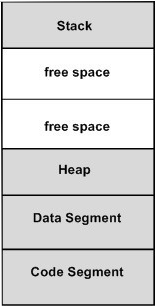
\includegraphics[scale=0.4]{images/memory}
    \end{tabular}
\end{frame}

\begin{frame}[fragile]
    \frametitle{Motivation}

    \begin{lstlisting}[language=C++, basicstyle=\footnotesize\ttfamily]
void add_2(int x){
    x += 2;
}

int main(){
    int x = 5;
    add_2(x);
    cout<<x<<endl;
    return 0;
}
    \end{lstlisting}

    \onslide<1-> \tabitem What would this code print?\\
    \onslide<2-> \tabitem Does the \texttt{add\_2} function work?\\
    \onslide<3-> \tabitem What can we do to make it work?\\
\end{frame}

\begin{frame}
    \frametitle{Pointers}
    
    \begin{itemize}
        \item A pointer is a data type that allow us to store the address of another variable.
        \item This way we don't keep track of the value of a variable, but \textit{where it is located in memory}.
        \item By knowing a variables location rather than value, we can access it from \textbf{anywhere} in the program.
    \end{itemize}

\end{frame}

\begin{frame}
    \frametitle{Pointers - How to use them}

    \textbf{When Declaring:}

    \texttt{<datatype> *<name> = \&<variable>;} \\
    \texttt{int *ptr = \&var}

    \textbf{When Using:}

    \texttt{*<name>} $\leftarrow$ The value of in the location in memory\\
    \texttt{<name>} $\leftarrow$ The location of the variable itself\\
    
\end{frame}

\begin{frame}[fragile]
    \frametitle{Pointers - What would this print?}
    
    \setlength{\tabcolsep}{15pt}
    \begin{tabular}{l l l}

        a)

        &

        \begin{lstlisting}[language=C++, basicstyle=\small\ttfamily]
int a = 5;
int *p = &a;
cout << *p << endl;
        \end{lstlisting}

        &

        \onslide<2->{5} \\[1cm]

        b)

        &

        \begin{lstlisting}[language=C++, basicstyle=\small\ttfamily]
int a = 5;
int *p = &a;
cout << p << endl;
        \end{lstlisting}

        &

        \onslide<3->{\texttt{0x0F032010}} \\[1cm]

        c)

        &

        \begin{lstlisting}[language=C++, basicstyle=\small\ttfamily]
int *p = 5;
cout << *p << endl;
        \end{lstlisting}

        &

        \onslide<4->{\texttt{ERROR}} \\
    \end{tabular}

\end{frame}

\begin{frame}[fragile]
    \frametitle{Referencing}

    \begin{itemize}
        \item In \texttt{C++} we can also create \textit{reference variables}.
        \item This will essentially give a new name to an already existing variable.
        \item \texttt{int \&r = a} $\leftarrow$ Anything that happens to \texttt{r} will happen to \texttt{a}.
        \item We can use it in \textit{functions} and solve the reference problem.
    \end{itemize}

    \setlength{\tabcolsep}{0.5cm}
    \begin{tabular}{l | r}
    \begin{lstlisting}[language=C++,basicstyle=\small\ttfamily]
void add_2(int &x){
    x += 2;
}
    \end{lstlisting}

        &

    \begin{lstlisting}[language=C++,basicstyle=\small\ttfamily]
void add_2(int *x){
    *x += 2;
}
    \end{lstlisting}

    \end{tabular}

\end{frame}

\begin{frame}
    \frametitle{In Review}

    \tabitem Each varaible is located in memory and has an address.\\
    \tabitem Pointers allow us to directly interact with memory addresses.\\
    \tabitem Referencing allows us to give new names to variables.\\[0.5cm]

    \texttt{int *p = \&a;} $\leftarrow$ Creates pointer \texttt{p} referencing \texttt{a}.\\
    \texttt{*p = 5;} $\leftarrow$ Updates the value in that location in memory.\\
    \texttt{p = \&b;} $\leftarrow$ Updates the position in memory \texttt{p} references.\\
    \texttt{int \&r = a;} $\leftarrow$ \texttt{a} can now be called as \texttt{r}.
\end{frame}

\section{The STL Library}

\begin{frame}
    \frametitle{Data Structures - Challenge}

	We want to write a program that stores a sequence of numbers and allows the following three operations

    \begin{itemize}
        \item Add an element to the front
        \item Add an element to the back
		\item Pop the element in the front
    \end{itemize}

	How would you do this?
\end{frame}

\begin{frame}
    \frametitle{Data Structures}

	\begin{center}
		How we store and process data will  affect significantly the performance and efficiency of out program.
	\end{center}

    \begin{itemize}
        \item A data structure is a way of organizing and processing data.
        \item It is like a blueprint that tells us how we should store and connect values, how these values should relate and the functions that we can apply to the data.
		\item Just like algorithms, data structures are an abstract concepts that we implement in our computer programs.
    \end{itemize}
\end{frame}

\begin{frame}
    \frametitle{What is \textbf{STL}?}

    \begin{itemize}
        \item \textbf{S}tandard \textbf{T}emplate \textbf{L}ibrary
        \item It is the name given to all the native C++ libraries.
        \item It works with any kind of variables.
        \item It is mainly made up of:
            \begin{itemize}
                \item[--] Containers
                \item[--] Algorithms
                \item[--] Functions
                \item[--] Iterators
            \end{itemize}
    \end{itemize}
\end{frame}

\begin{frame}
    \frametitle{Vector}

    \begin{itemize}
        \item A vector is a structure of dynamic size that stores data sequentially, assigning an index to each element.
        \item It is basically a more powerful implementation of the native \texttt{C++} \textit{array}.
    \end{itemize}

    \begin{center}
        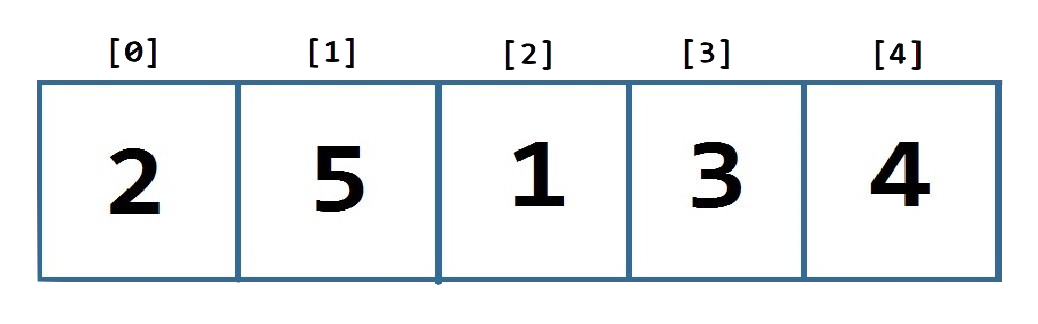
\includegraphics[scale=0.25]{images/vector}
    \end{center}
\end{frame}

\begin{frame}
    \frametitle{Common Functions}

    \begin{itemize}
        \item \texttt{size} : Returns size of vector
        \item \texttt{clear} : Erase all elements inside the vector
        \item \texttt{push\_back} : Insert an element to the back
        \item \texttt{pop\_back} : Erase the last element
        \item \texttt{insert} : Insert element in any position
        \item \texttt{erase} : Erase an element in any position
        \item \texttt{empty} : Returns \texttt{true} if the vector is empty
        \item \texttt{front} : Access first element
        \item \texttt{back} : Access last element
    \end{itemize}
\end{frame}

\begin{frame}
    \frametitle{Deque}
    
    \begin{itemize}
        \item A \textit{deque} is the \texttt{C++} implementation of a \textit{list}.
        \item It is similar to a vector but some of its \textit{methods} have different \textit{complexities}.
        \item It has two additional functions:
            \begin{itemize}
                \item[--] \texttt{push\_front} : Insert an element at the beginning.
                \item[--] \texttt{pop\_front} : Erase the first element.
            \end{itemize}
    \end{itemize}

    \begin{center}
        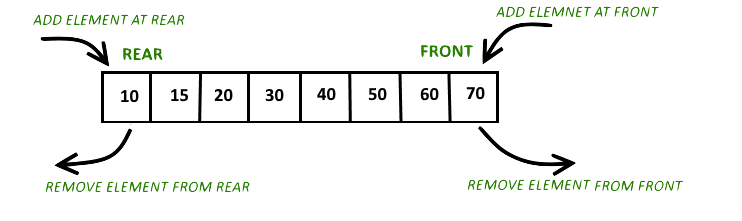
\includegraphics[scale=0.4]{images/deque}
    \end{center}
\end{frame}

\begin{frame}[fragile]
    \frametitle{Deque - Example}

    \begin{lstlisting}[language=C++]
int main(){
    deque<int> myDeque = {1,2,3,4,5};
    myDeque.push_front(6);
    myDeque.push_front(0);
    myDeque.push_front(7);
    myDeque.pop_front();
    for(int i = 0 ; i < myDeque.size() ; i++){
        cout << myDeque[i] << ' ';
    }
    return 0;
}
    \end{lstlisting}

    \begin{tcolorbox}[title=Output,fontupper=\scriptsize,fonttitle=\scriptsize]
        \onslide<2->{\texttt{0 6 1 2 3 4 5}}
    \end{tcolorbox}
\end{frame}

\begin{frame}
    \frametitle{Stack}
    
    \begin{tabularx}{\linewidth}{m{0.62\linewidth}  m{0.3\linewidth}}
        \begin{itemize}
            \item A stack is a data structure that in which we can only access to the last element added.
            \item It can be seen as a restricted deque.
            \item It has the following methods:
                \begin{itemize}
                    \item[--] \texttt{empty} : Is the stack empty?
                    \item[--] \texttt{size} : Returns the stacks size.
                    \item[--] \texttt{top} : Returns the top element.
                    \item[--] \texttt{push} : Inserts new element.
                    \item[--] \texttt{pop} : Erase the element on top.
                \end{itemize}
        \end{itemize}

        &

        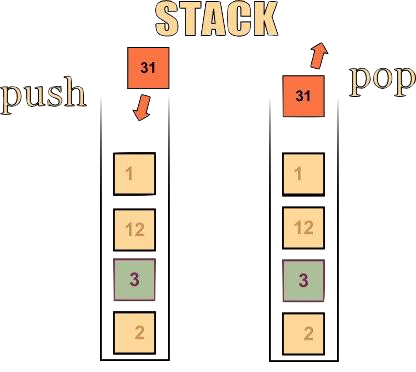
\includegraphics[scale=0.25]{images/stack}
    \end{tabularx}

\end{frame}

\begin{frame}[fragile]
    \frametitle{Stack - Example}

    \begin{lstlisting}[language=C++]
int main(){
    stack<int> myStack;
    myStack.push(1);
    myStack.push(2);
    myStack.push(3);
	myStack.pop();
	while(!myStack.empty()){
        cout << myStack.top() << ' ';
        myStack.pop();
    }
    return 0;
}
    \end{lstlisting}

    \begin{tcolorbox}[title=Output,fontupper=\scriptsize,fonttitle=\scriptsize]
        \onslide<2->{\texttt{2 1}}
    \end{tcolorbox}
\end{frame}

\begin{frame}
    \frametitle{Queue}

    \begin{itemize}
        \item A queue is a data structure in which we can only access the oldest element.
        \item It can be seen as a restricted deque.
        \item It has the same methods as \textit{stack}, with the only differences being in \texttt{push} and \texttt{pop}.
    \end{itemize}

    \begin{center}
        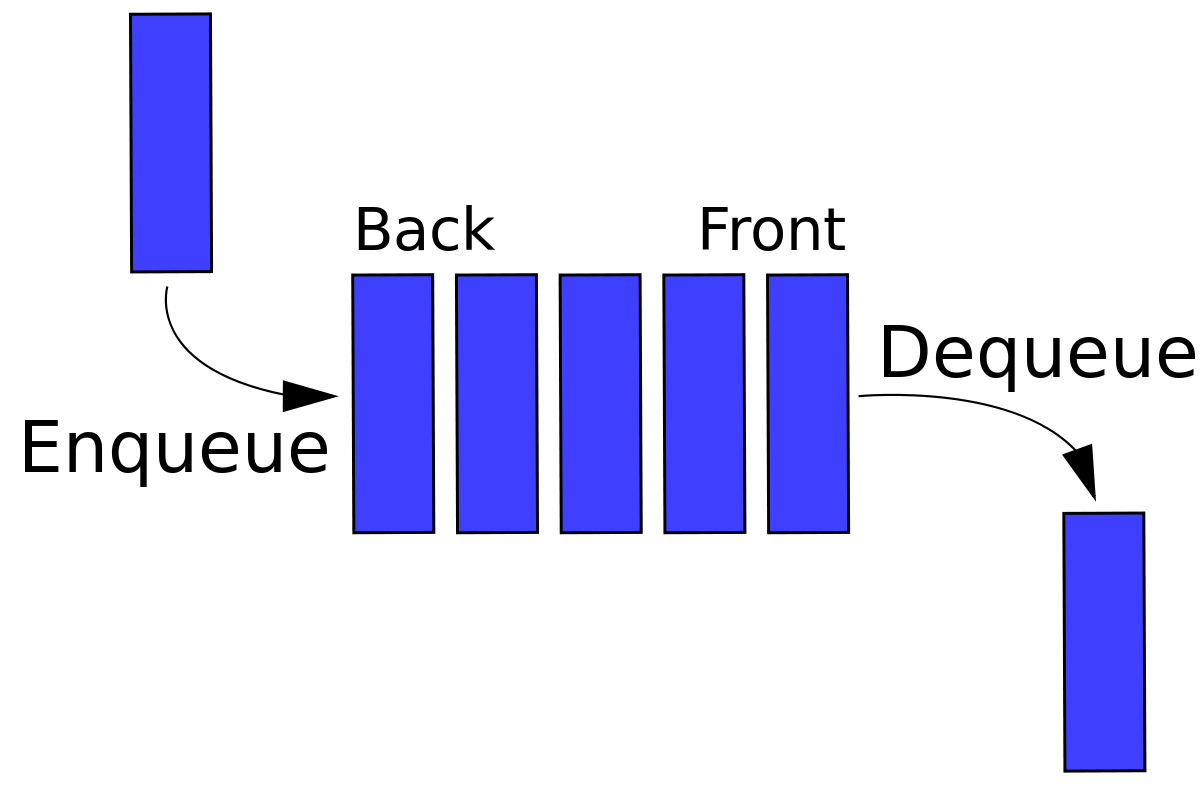
\includegraphics[scale=0.1]{images/queue}
    \end{center}
\end{frame}

\begin{frame}[fragile]
    \frametitle{Queue - Example}

    \begin{lstlisting}[language=C++]
int main(){
    queue<int> myQueue;
    myQueue.push(1);
    myQueue.push(2);
    myQueue.push(3);
	myQueue.pop();
	while(!myQueue.empty()){
        cout << myQueue.front() << ' ';
        myQueue.pop();
    }
    return 0;
}
    \end{lstlisting}

    \begin{tcolorbox}[title=Output,fontupper=\scriptsize,fonttitle=\scriptsize]
        \onslide<2->{\texttt{2 3}}
    \end{tcolorbox}
\end{frame}

\begin{frame}
    \frametitle{Map}

    \begin{itemize}
        \item A data structure that associates a key to a value.
        \item It is like a vector, but the key can be any kind of datatype and have no particular order.
        \item The key and the value can have different datatypes.
        \item Declaration: \texttt{map<key type, value type>}
    \end{itemize}

\end{frame}

\begin{frame}[fragile]
    \frametitle{Map - Example}

    \begin{lstlisting}[language=C++, basicstyle = \scriptsize\ttfamily]
int main(){
    map<int,string> myMap;
    myMap.insert({1,"World"});
    myMap[0] = "Hello";
    myMap[2] = "Lorem Ipsum";
    cout << myMap.size() << "\n";
    for(auto i:myMap){
        cout << i.first << ' ' << i.second << "\n";
    }
    return 0;
}
    \end{lstlisting}

    \begin{tcolorbox}[title=Output,fontupper=\scriptsize,fonttitle=\scriptsize]
        \onslide<2->{\texttt{0 Hello\\
            1 World\\
            2 Lorem Ipsum\\
            The map is empty
        }}
    \end{tcolorbox}
\end{frame}

\begin{frame}
    \frametitle{Other Structures}

    \begin{itemize}
        \item \texttt{priority\_queue}
        \item \texttt{set}
        \item \texttt{unordered\_set}
        \item \texttt{multiset}
        \item \texttt{unordered\_map}
        \item \texttt{multimap}
        \item \texttt{pair}
        \item \texttt{tuple}
    \end{itemize}
\end{frame}

\begin{frame}
    \frametitle{Algorithms - \texttt{std::sort}}

    \begin{itemize}
        \item The \texttt{sort} algorithm allows us to sort containers very quickly.
        \item It is usally used on \textit{vectors} and \textit{arrays}
        \item \texttt{sort(start address, end address, comparator)}
        \item There are very few cases in which we should implement our own sort.
        \item Sort works over the container, it doesn't return a copy but actually swaps elements.
        \item \textbf{Ex.}  \texttt{sort(vec.begin(), vec.end());}
    \end{itemize}
\end{frame}

\end{document}
